\chapter{案例分析}
\section{数据介绍}
我们所用的数据来源于松浦MC-510V加工中心的具体操作数据(见图3.1)。\par
% 
\begin{figure}[htp]
    \centering
    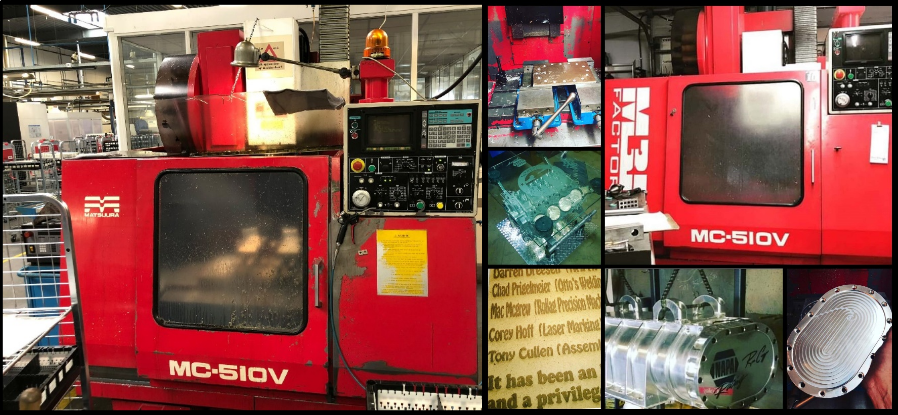
\includegraphics[width=14cm]{Chapter3/machine.png}
    \caption{松浦MC-510V加工中心}
\end{figure}
% 
% 
在操作过程中,我们采用传感器技术,利用声音传感器、振动传感器、电流传感器对不同操作条件下的铣床运行进行观察与记录,得到了在常规切削、进口切削以及出口切削时的刀具磨损相关数据,并将这些数据实时写入Matlab的mill.mat文件中(见图3.2)。\par
\href{https://github.com/QianZeHao123/OpenIE/tree/main/nc_machining_center/DATA}{完整数据:https://github.com/QianZeHao123/OpenIE/nc\_machining\_center/DATA}\par
% 
\begin{figure}[htp]
    \centering
    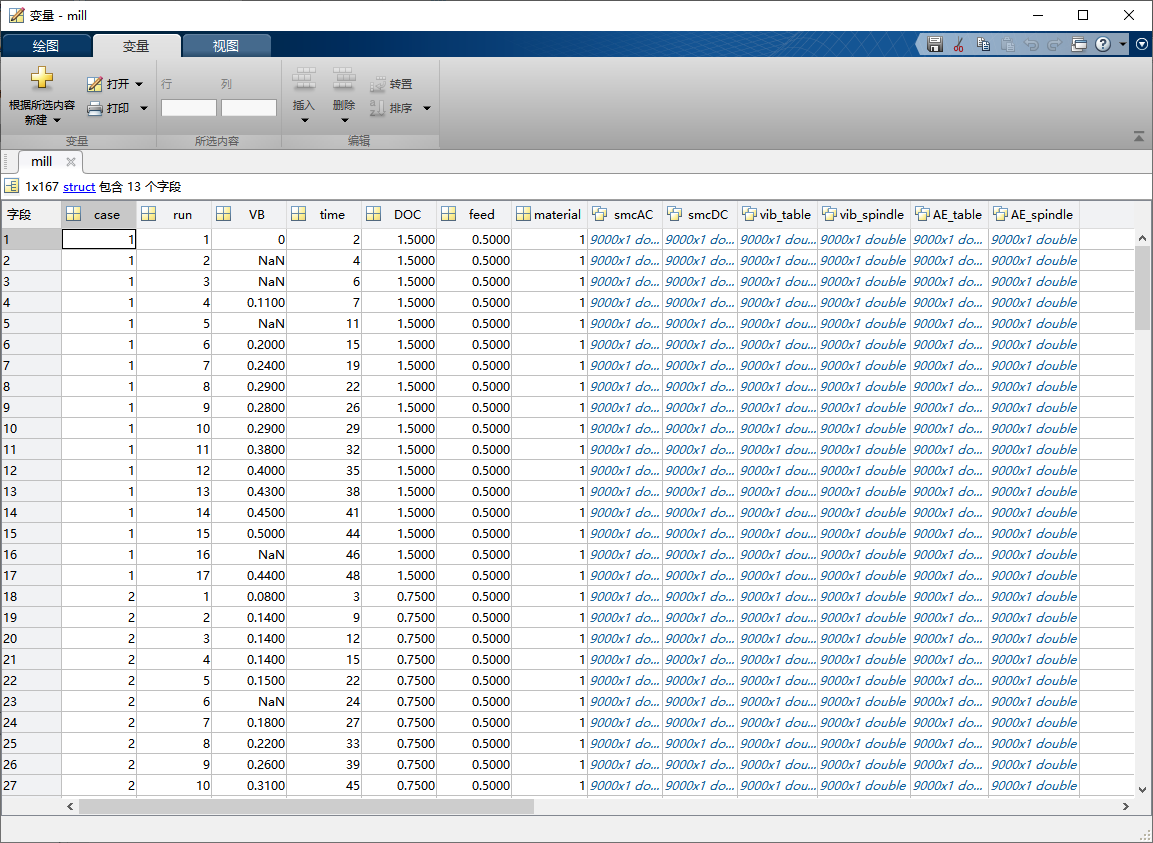
\includegraphics[width=14cm]{Chapter2/mill.png}
    \caption{Matlab mill中的数据}
\end{figure}
% 
% 
% 
\section{数据处理}
% 
由于我们训练刀具磨损量测定神经网络模型使用的是个人PC,配置如下:CPU(Intel(R) Core(TM) i5-9400F CPU @ 2.90GHz),GPU(NVIDIA GeForce GTX 1660),内存8.0 GB。一些几万参数的中大型神经网络模型无法在这种低算力的个人设备上进行训练,因此本项目中一组9000个数据的车床电流、震动和噪声信号无法被直接当做参数输入神经网络,故我们决定使用特征工程的方法,对6组采集的信号进行时域、频域分析,大大减少输入数据的量,并对分析后的数据进行筛选,选取对模型较为敏感的特征。\par
我们团队使用Matlab编写绘制了所有输出信号的脚本,用于人工筛选可以用来被训练的数据。在mill.mat文件中,共收集有167组数据,其中有21组数据中缺少刀具磨损量VB,因此不能被列入训练集,同时还有一组数据通过图像发现AC/DC电压出现 $ 10^{29} $ 异常,可能是由于信号传感器出现问题。经过人工观察图像筛选训练用信号,共有145组可被用于训练集。
\href{https://github.com/QianZeHao123/OpenIE/blob/main/nc_machining_center/draw_pic.m}{(145组信号图形并未上传GitHub,可通过运行OpenIE/nc\_machining\_center/draw\_pic.m脚本进行图像绘制)}\par
% 
\begin{figure}[htp]
    \centering
    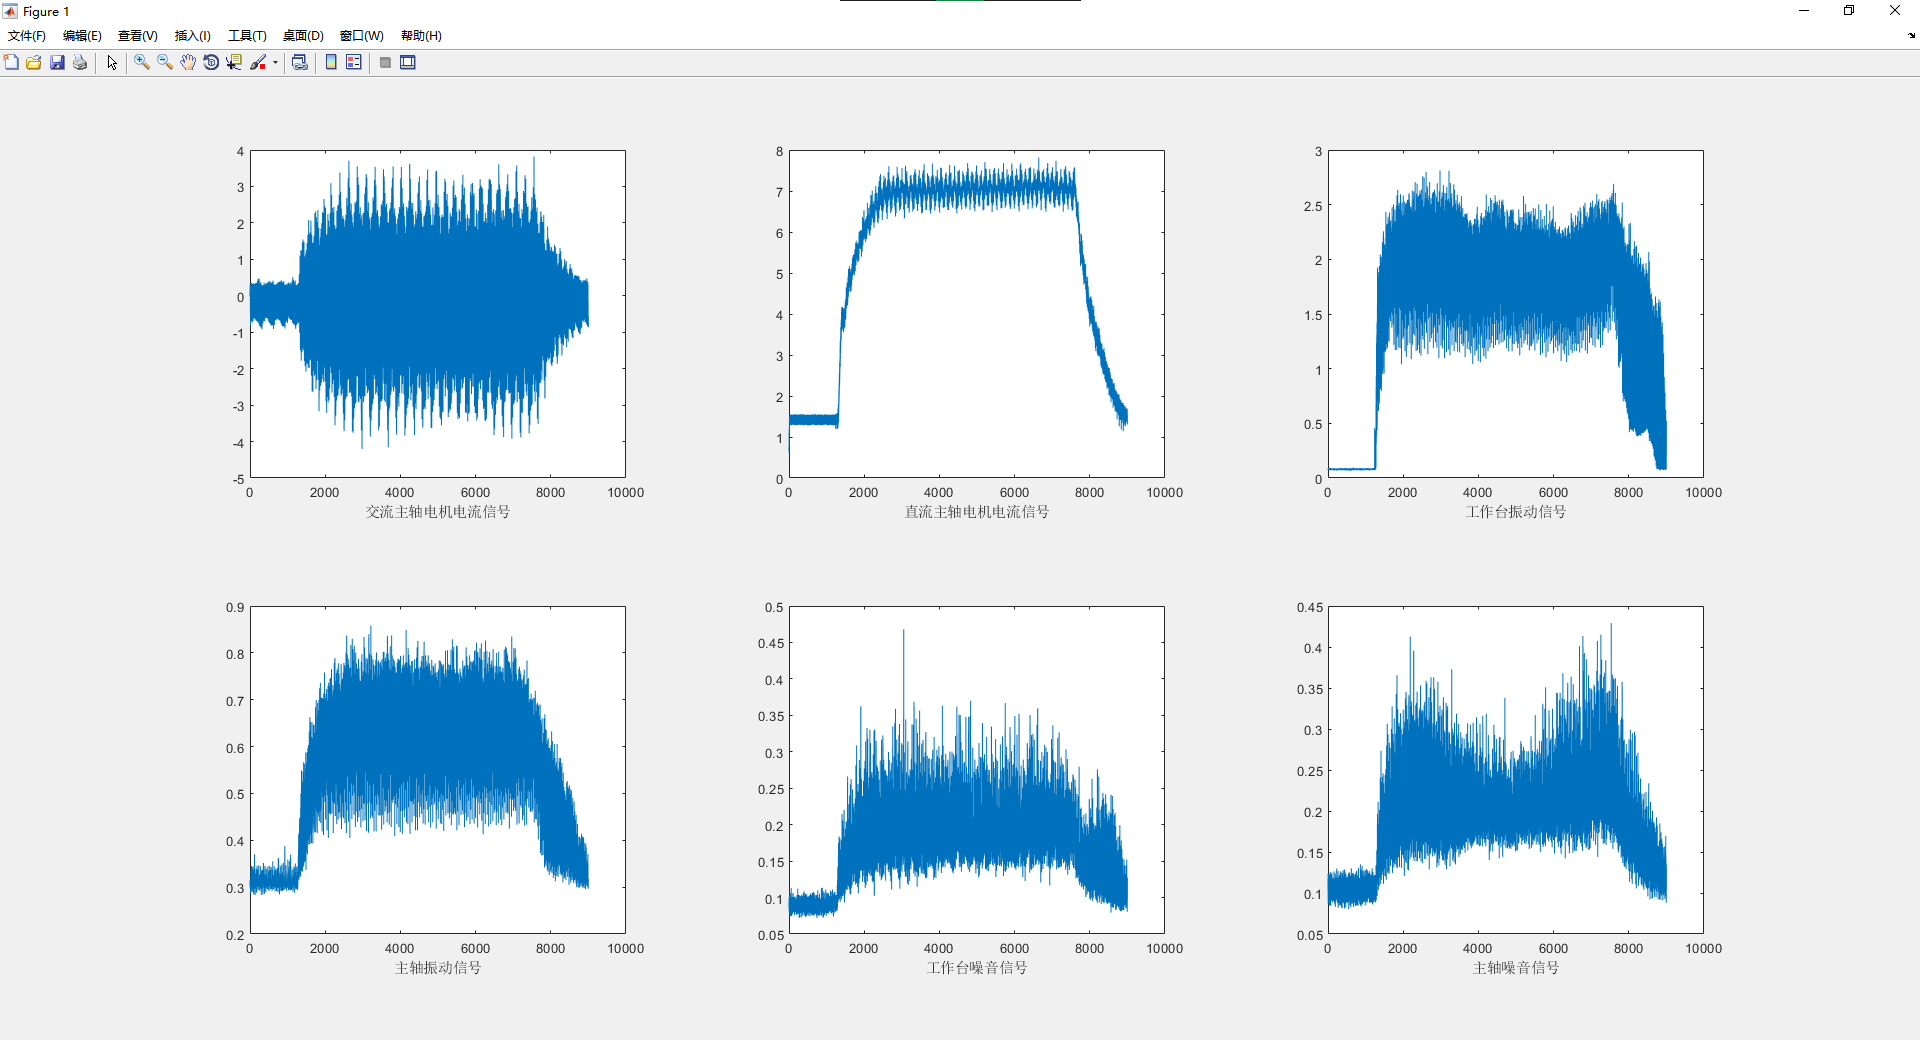
\includegraphics[width=14cm]{Chapter2/signal.png}
    \caption{机床传感器信号图像}
\end{figure}
% 
% 
% 
\section{神经网络训练}
经过数据筛选和特征工程,共获得145组数据,每组数据有60个参数,我们使用Matlab编写脚本,将这些数据转化为145rows~*~60colums的矩阵作为训练神经网络的输入(见图3.4),输出为与145组数据的相对应的刀具磨损量VB的值。\par
除了实现RNN中的隐藏状态使用的是PyTorch框架之外,为了提升训练效果,剩余部分采用MatLab实现。我们构建单隐藏层的Back Propagation神经网络,优化算法采用的是Bayesian Regularization,该算法相较于其他神经网络拟合训练时间更长,同时训练后的模型准确度更高,经过1min57s的训练在第602~iteration时模型达到最优,最小梯度达到 $ 9.92 \times 10^{-8} $,机器停止训练,具体结果如下(见图3.5)。
\footnote{本部分使用到了Matlab神经网络工具箱,需要Matlab版本不低于R2018 a,已使用Embedded Coder将NN toolbox训练过程转化为Matlab,\href{https://github.com/QianZeHao123/OpenIE/blob/main/nc_machining_center/neural_network_train.m}{代码链接点击此跳转}}
% 
% 
\subsection{神经网络超参数优化}
为提高神经网络的训练速度,节省一定的训练成本,提高网络的性能,需要对神经网络的超参数进行优化,我们实验中使用到了MatLab中的贝叶斯网络工具箱,贝叶斯优化能够结合过去的评估结果,在较短的时间内找到适合的超参数。\par
贝叶斯优化的原理是:使用贝叶斯定理先估计目标函数的后验分布,进而根据分布选择下一个要采样的超参数组合。上述方法充分利用了之前的采样点完善了目标函数的形状,从而能够找到全局最优的超参数。\par
% 
\subsection{BP神经网络模型部署}
训练好后的神经网络模型,投入实际生产中,可以通过运行\href{https://github.com/QianZeHao123/OpenIE/blob/main/nc_machining_center/neural_network_deploy.m}{Matlab(neural\_network\_deploy点击跳转)}这个脚本,输入可以为实时从机床传感器中获取的电压、噪声和震动信号,经过特征处理后转化成的60个参数,就可以根据获得的机床信号特征数据,预测当前刀具的磨损状况。\par
工业上,能运行Matlab脚本的机器一般对性能和存储要求比较高,在机床设备上部署神经网络算法需要将Matlab代码转化为性能高的C/C++,这里我们用到了Coder这个工具箱进行代码和模型转换,具体操作详见第五章工业应用:模型部署。\par
% 
% 
\begin{figure}[htbp]
% \centering
\begin{minipage}[t]{0.48\textwidth}
\centering

\includegraphics[width=6.5cm]{Chapter3/MLP.png}
% \label{fig_22}
\caption{神经网络结构图}
\footnote{输入层实际有60个参数,由于篇幅限制神经网络图中只绘制了9个,隐藏层节点实际为20个,图中只绘制了4个}
\end{minipage}
\begin{minipage}[t]{0.48\textwidth}
\centering
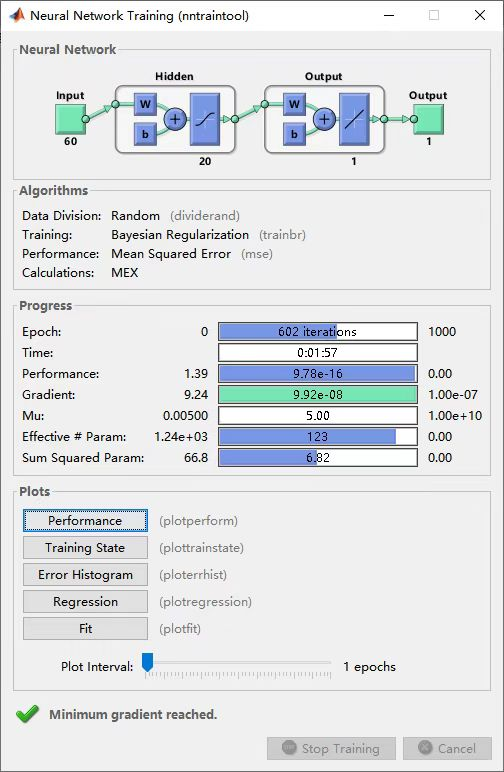
\includegraphics[width=5.5cm]{Chapter2/res.jpg}
\caption{使用MatLab神经网络工具箱进行全连接层训练}
% \label{fig_23}
\end{minipage}
\end{figure}
%
% 